In the previous chapters, we only considered uni-variable functions, i.e. functions that takes one number as input.  However, in practice, the quantities we are interested in may be related to serveral variables.  For example, suppose we would like to know our net income $I$ in manufacturing and selling a type of product.  The net income would depend on several variables, including the unit cost for manufacturing the product ($C$), the unit price of the product ($P$), and the quantity of product sold ($Q$).  Therefore, we have 
\[I = (P-C)Q := g(P,C,Q)\]
Here, $g$ would then be a function that takes three numbers as input.  

Previously when we set out to visualize a uni-variable function, say $f(x)$, we would plot $y = f(x)$ on a Cartesian plane using curve sketching techniques.  For functions of several variables, when the number of inputs is greater of equal to $3$, then it is quite challenging to visualize the function.  However, in the special case where the number of inputs is $2$, i.e. a function like $f(x,y)$, we can visualize the function by plotting $z = f(x, y)$ as a three-dimensional surface, where the two inputs $x$, $y$ serve as the $x$- and $y$-coordinates, and the function value $f(x,y)$ serves as the $z$-coordinate.  With the advent of computer graphics, graphing a 3-D plot has been easier than ever (eg. using Wolfram on-line services).  However, in absence of 3-D graphing utilities, we can still figure out how the function approximately looks like using the following techniques

\begin{enumerate}
    \item \underline{Traces on planes parallel to the $yz$- and $xz$-plane}: When the $x$ input in $f(x, y)$ is treated as a fixed constant $x_0$, we have $z = f(x_0, y)$, which now becomes a uni-variable function that can be plotted on a Cartesian plane.  The curve plotted is actually the trace of $f(x, y)$ when sectioned with the plane $x = x_0$, which is a plane perpendicular to the $x$-axis.  For example, in the left panel of the graph below, the section made by $x = x_0$ results in a trace of a parabola.  Similarly, we may treat the $y$ input as a fixed constant $y_0$, which results in a trace of the surface sectioned by $y=y_0$, a plane perpendicular to the $y$-axis. 
    \item \underline{Contour map}: We can also section the surface along planes that are parallel to the $xy$-plane.  That is, for a given value of $z_0$, we find all points $(x,y)$ that satisfied $f(x,y) = z_0$ and graph the trace on the Cartesian plane.  What is great about contour map is that, as long as the function $f(x,y)$ is differentiable everywhere (we will talk about the derivatives for functions of several variables in a bit), we can pick a bunch of possible values of $z$ and graph all their section traces on the $xy$-plane, and these traces would not intersect with each other.  For example, in the right panel of the graph below, the section traces for $z=1, 2, 3, 4$ are graphed on the Cartesian plane, which form a bunch of concentric circle.  Also notice that although we are plotting traces of equal spacing of $z$, the concentric circle are closer and closer to each other as $z$ gets larger.  This implies that the surface is steeper far away from the origin point and gentler near the origin point.  This kind of plot is called the contour map, and is widely used in geographic maps. 
\end{enumerate}

\begin{figure}[ht]
    \centering
    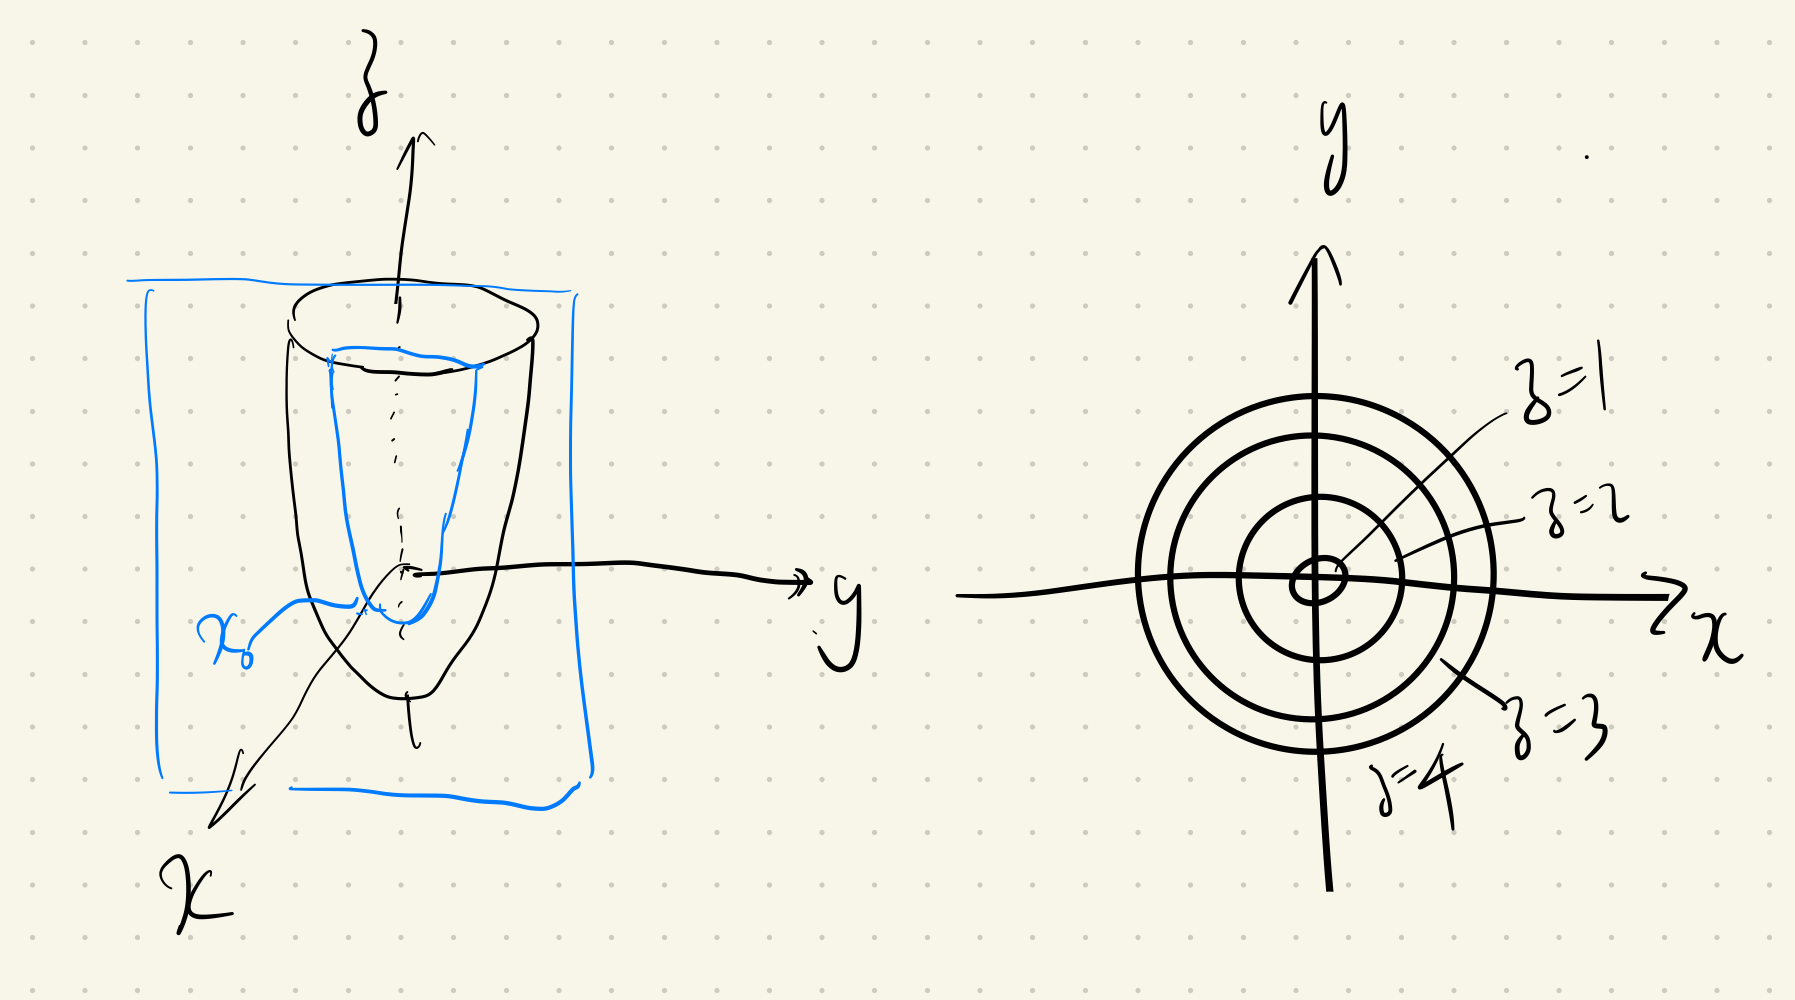
\includegraphics[width = 0.7\textwidth]{figures/chap 08/3D-graph.png}
\end{figure}

\subsection{Partial derivatives of a function of two variables}
When we were dealing with univariable functions, we used derivatives to evaluate the slope of their tangent lines at a certain point, which reflects the rate of change of these functions at that very point.  In functions of two variables, we can still try to evaluate the rate of change of these functions.  What is different from univariable functions is that, for a univariable function, say, $f(x)$, when we are moving a tiny bit away from $(x_0, f(x_0))$, we can only go to $(x_0 + \delta x, f(x_0+ \delta x))$ or $(x_0 - \delta x, f(x_0 - \delta x))$, both of which have the same rate of change relative to $(x_0, f(x_0))$ as long as $f(x)$ is continuous.  However, for a function of two variables, say, $g(x,y)$, for every point on the surface $(x_0, y_0, f(x_0, y_0))$, there are countless direction we can move away from this point, and each direction would have a different rate of change.  Therefore, before we evaluate the derivative of a fucntion of two variables, we have to specify which direction are we moving away from the point of interest.  Two most obvious directions are along the $x$-axis (holding the $y$-coordinate as constant) and along the $y$-axis (holding the $x$-coordinate as constant).  These directions lead to the two first-order partial derivatives of the function, defined as below:

\begin{defi}[First-order Partial Derivatives]{}
    Let $f(x,y)$ be a continous function, then the first partial derivative of $f$ with respect to $x$ and $y$ are defined as
    \begin{align*}
        \frac{\partial f}{\partial x} := f_x(x,y) &:= \lim_{h \rightarrow 0} \frac{f(x+h,y)-f(x,y)}{h}\\
        \frac{\partial f}{\partial y} := f_y(x, y) &:= \lim_{h \rightarrow 0} \frac{f(x,y+h)-f(x,y)}{h}\\
    \end{align*}
\end{defi}

Luckily, although this definition seems cumbersome, the way to evaluate partial derivatives is to simply treat the input that is not to be differentiated as constant.  For example, suppose we let $f(x, y) = 2x + 3xy + 1$, then the partial derivative of $f$ with respect to $y$ is
\[\frac{\partial f}{\partial y} = 0 + 3x + 0 = 3x\]